\documentclass{article}


\usepackage{arxiv}

\usepackage[utf8]{inputenc} % allow utf-8 input
\usepackage[T1]{fontenc}    % use 8-bit T1 fonts
\usepackage{hyperref}       % hyperlinks
\usepackage{url}            % simple URL typesetting
\usepackage{booktabs}       % professional-quality tables
\usepackage{amsfonts}       % blackboard math symbols
\usepackage{nicefrac}       % compact symbols for 1/2, etc.
\usepackage{microtype}      % microtypography
\usepackage{lipsum}		% Can be removed after putting your text content

\usepackage[toc,page]{appendix}
\usepackage{amsmath}
\usepackage[ruled ]{algorithm2e}
\usepackage{tikz}
\usetikzlibrary{fit,positioning,arrows,automata,calc}
\tikzset{
	main/.style={circle, minimum size = 5mm, thick, draw =black!80, node distance = 15mm},
	invis/.style={circle, minimum size = 10mm, thick,  node distance = 15mm},
	connect/.style={-latex, thick},
	box/.style={rectangle, draw=black!100}
}

%TODO rechtschreibung überprüfen
% TODO groß und kleinschreibung, z.b Kalman filter vs Kalman Filter und Section vs section, etc.

\title{Bachelor Project Report: \\ Multi-Object-Pose-Tracking on Point Detections}

%\date{September 9, 1985}	% Here you can change the date presented in the paper title
%\date{} 					% Or removing it

\author{
  Simon Giebenhain\thanks{The work was done as a Bachelors Project supervised by Prof. Bastian Goldlücke} \\
  Department of Computer Science\\
  University of Constance\\
  \texttt{simon.giebenhain@uni-konstanz.de} \\
}

\begin{document}
\maketitle

\begin{abstract}
%TODO
\end{abstract}


% keywords can be removed
%\keywords{First keyword \and Second keyword \and More}


\section{Introduction}


\subsection{Multi-Object Tracking}

Multiple Object Tracking (MOT), also known as Multi-Target Tracking, refers to the task of identifying and maintaining the identities of objects of interest over time. Usually MOT is performed on video data, as the most common use cases are sports tracking, tracking of pedestrians and other traffic participants for surveillance purposes. Especially autonomous driving heavily depends on solid MOT software. Despite the fact these applications are of particular interest for the industry and an active reasearch filed, MOT remains a challenging task and an interesting research topic.


\subsection{The Specific Task at Hand}

The methods presented in this paper are tailored towards MOT on specific three-dimensional bird trajectories. Next to the location also the orientation in three-dimensional space of the birds are being tracked. The data is described in detail in \ref{data_setup} and \ref{data_noise}.\\
This work particularly aims at providing accurate 3d bird trajectory data for the  analysis of the collective behaviour of birds at the department for Collective Behaviour from the Max Planck Institute and the University of Konstanz. The research group is using the  \href{https://www.vicon.com/software/tracker/}{VICON Tracker 3} system
to record the trajectories of multiple birds at once. However the acquired trajectories are of bad quality. The trajectories have a lot of holes and ID-switches between birds occur frequently. This work aims at building coherent 3d trajectories. The trajectories are built from unlabelled 3d detections. 
For the behaviour analysis of birds ID-switches are fatal. Therefore my approaches take special care of maintaining the identities of birds without switching them.



\subsection{Data Capturing Setup}
\label{data_setup}
% markers humanly designed, room for improvement


%TODO marker setup 
This section explains how the data is captured, which is used as input to the tracking algorithm. 
The data was captured inside of a large barn with a 2D array of infrared cameras filming downwards from above. Each bird is equipped with a tiny backpack which has space for 4 infrared reflecting markers, positioned in a unique pattern. There can be small elevations on the backpack, meaning that the specified pattern can be three-dimensional instead of just lying in one plane. Using these patterns enables to predict the orientation of the birds in three-dimensional space. These patterns are specified by hand by the supervisers of the experiment. An analysis of the performance of different patterns could lead to insights which allow for the design of better patterns. However such proceedings are out of scope for this work and may be subject to future research if need be.

The aforementioned infrared cameras feed information directly to the VICON Tracker3 system, which puts all detections into a unified three-dimensional coordinate system. The input to the tracking algorithms presented here is therefore a set of unlabelled 3d detections for each time frame. The VICON system produces detections accurate to the millimeter. Therefore this work assumes that there is little noise in the true positive(TPs) detections.

 Although the room was painted such that a minimal amount of infrared light gets reflected from anything else than the infrared markers, there is still a substantial amount of false positive (FPs) detections. Similarly there are lots of false negatives (FNs), especially when the birds are moving and occluding the markers with their wings. Some more details on the noise in the data is given in \ref{data_noise}.


\subsection{Exploring the Data}
\label{data_noise}
% e.g. fps
% different kind of noise present
% Unfortunately no ground truth to evaluate results, other than simulated data

%TODO: some topdown screenshots, showing differnt noise present to show false positives and false negatives

%TODO some number from KF

As stated in the previous sections there is a lot of noise in the data. In this section I want to provide evidence for that claim...



\section{Related Work}
% research focuses on pedestrians,  and visual similarity, pose is uncommon, solely position no rotation
% reference 3D-Kalmanfilter paper to support choice of Klaman Filter
% check tracking the trackers and summarize some common approaches

% MILAN_RNN tries to tackle the problems in a unified framework
% Cite some interesting other appraoches


Multiple-Object Tracking partly is so challenging, because of the great variety of information present. Usually scenes are very busy, there can be an arbitrary number of objects of interest present and the camera position can change. As a result most approaches follow a \emph{tracking-by-detection} scheme, where an object detector locates objects of interest in each frame. This way the algorithm can focus on the information around the detected objects and discard information which seems irrelevant. The challenge is then to assign the detections to the tracks. This procedure is called \emph{detection to track assignment} and is the most crucial point of modern MOT algorithms. \\
This work naturally follows a \emph{tracking-by-detection} scheme, since the only available data are 3d detections.

%TODO I should explain tracking by detection
Despite the great success of deep learning in most computer vision tasks over the past years, deep learning is only slowly improving MOT methods. \cite{milan_rnn_tracking} reason why applying deep learning to MOT is far from trivial. In MOT the tracked states are continuous, whereas the detection-to-track-assignment is a discrete assignment problem. The number of tracked objects is arbitrary and death and birth of tracks have to be handled. These circumstances make it hard to design a architecture which can handle this variety of data.

%TODO: look at popular papers
%TODO: also cite 3d Kalman Filter paper
Therefore most research papers follow the \emph{tracking-by-detection} scheme and construct elaborate similarity measures to solve the \emph{detection-to-track-assignment}. 
%TODO maybe link with following paragraph and move that paragraph up

\subsection{Differences to other works}
%TODO bird and death, we know how many birds in each scene, 

Most of the MOT literature focuses on tracking pedestrians, as surveillance and autonomous driving are two industry applications for MOT which drive research. Additionally the majority of research uses visual appearance features in order to make the \emph{detection to track assignment}. They do so for good reason, as \cite{tracking_the_trackers} found that the most defining feature of the best performing models on the MOT15 benchmark (\cite{MOT15}) and MOT16 benchmark (\cite{MOT16}) is a good affinity measure using appearance features.

My task differs substantially from the majority of modern approaches to MOT. The methods presented here use no visual data and the usual \emph{detection to track assignment} is not sufficient to obtain good tracks. Since each bird has 4 markers, an exact \emph{detection to marker assignment} is necessary, especially to estimate the orientation well. \\
This task is complicated by a high rate of FPs and an even higher rate of FNs in the detections of the VICON system. Robustness to such noise is the main goal of this work.

%TODO name paragraph, something like focus of this work
The difficulties of my task deviate from the difficulties tackled in research. In the literature the main focus lies on modeling affinity in order to solve the \emph{detection to track assignment}. Clearly visual appearance is the richest source of information to that regard. Usually a strong affinity model is needed when working on detections in crowded scenes which are heavily troubled by occlusion. For this reason there is little research working on mere point detections.\\
In the setup presented here detections are three-dimensional and have a very high precision. This resolves occlusion problems and hence the \emph{detection to track assignment} is easy in most cases, since a Kalman Filter with a constant velocity motion model is able to maintain the identity of birds, as can be seen in section \ref{results_kalman_filter}.
There are, however, two challenges remaining:
While the \emph{detection-to-track-assignemnt} is easy, the \emph{detection to marker assignment} remains challenging. False positive detections have also be identified as such. A correct detection to marker assignment is crucial, in order to accurately predict the orientation, as a false assignment heavily disrubts the orientation estimation. This task becomes especially challenging when less than 3 markers are detected and when FPs are present at the same time. This problem becomes worse when the birds are moving and the detection quality deteriorates for multiple consecutive frames.
Second, maintaining tracks over periods with no detections at all. In the most extreme cases predicting a correct orientation is almost impossible, but this can be tolerated, as long as the position predictions for multiple future steps are similar to the actual movement of the bird. Then the position of such a track can be corrected as soon as a single detection of the bird reappears. Over such periods the orientation estimation can inevitabily become inaccurate. Maintaining an accurate postion prediction is especially important since initializing new tracks has to be done with extreme precaution, since ID-switches are not tolerated. Therefore it is crucial to identify the detected pattern with a high certainty, before continuing the tracking of the bird corresponding to the detected pattern. False positive detections are frequent and with no prior information about the position of a bird it is difficult to identify FPs as such. Therefore it is important to have 4 true positive detections which match  the pattern of a missing birds exactly. Sometimes it can take hundreds of steps for such an occasion to occur. Therefore losing a track is very costly. %TODO find examples and check if it is actually true
%TODO If I extend createNewTrack() to work with 3 dets, make sure to update text

\subsection{Problem Formulation and Notation}
\label{problem_def}
%TODO should I move dat cupturing setup here???
%TODO move unneccerssary stuff to other sections and make this one as precise as possible

This section introduces the notation used in the following section while stating the problem mathematically. The task is to estimate the position and orientation at every timestep for every object. \\
Conventually the MOT problem is formulated in such a way that the number of present objects can vary from frame to frame. The approaches presented in my work do are capable of handling a varying number of objects, provided that the patterns of each object which can possible become visible in the scene is known beforehand. For the sake of simplicity I formulate the problem with a fixed number of objects $N$, as this is the case for the bird data, which is the main focus of this paper.\\
Each of these $N$ objects is equipped with a pattern made up out of $K$ markers. Let the pattern of the $n\text{-th}$ object be denoted by $m^{(n)} = 
\begin{pmatrix}
m^{(n)}_1 \\
\vdots \\
m^{(n)}_K
\end{pmatrix} \in \mathbb{R}^{Kxd}$, where the $k\text{-th}$ row holds the $k\text{-th}$ marker, $m^{(n)}_k$.

Let $T$ be the number of total timesteps, then the input is a sequence of detected point clouds denoted by $\left( \mathcal{X}^{(t)} \right)_{t=1}^T$, where $\mathcal{X}_t \subset \mathbb{R}^d$. 
%TODO where to put this 
While it would be possible to formulate the problem and solutions with $d$ beign arbitrary, I constrain my work to $d=3$, as this case seems to have the most applications. It is important to note here that $\mathcal{X}^{(t)}$ is a set of $d$ dimensional points, meaning that we have no prior information which detection belongs to which object or to which marker of which object. As explained in section \ref{approaches} not knowing the detection to marker assignment is the most critical point of this problem. While conceptually $\mathcal{X}^{(t)}$ is a set, the detections are stored in such a way that there is an arbitrary ordering to them. I will reference the corresponding but ordered detections with $X^{(t)}$. \\
Furthermore each object is equipped with a pattern

The values to estimate are the position trajectories for each object $\left(p^{(t)}_1\right)_{t=1}^T, \dots,\left(p^{(t)}_N\right)_{t=1}^T$ and the rotations $\left(r^{(t)}_1\right)_{t=1}^T, \dots,\left(r^{(t)}_N\right)_{t=1}^T$. 
%TODO: where to put this (https://pdfs.semanticscholar.org/b12a/a54a6676f2e2614c8d463334799d6cfdb93e.pdf says the other way around and http://read.pudn.com/downloads182/ebook/848457/Wiley.Global.Positioning.Systems.Inertial.Navigation.and.Integration.2nd.Edition.Jan.2007.pdf)
For $d=3$ there are many common way to represent rotations, next to the canonical repsentation as a rotation matrix, there are for example Euler angles and quaternions. Euler angles are a minimal representation since it only requires 3 parameters. However they exhibit singularities, which correspond to a gimbal lock configuration, where large changes in the euler angles are required to represent small changes in the actual rotation, \cite{manifolds}. Therefore Euler angles are generally considered inferior to quaternions in controlling and tracking tasks. 

The task is to come up with estimates for the positions, $\left(\hat{p}^{(t)}_1\right)_{t=1}^T, \dots,\left(\hat{p}^{(t)}_N\right)_{t=1}^T$, and rotations, $\left(\hat{r}^{(t)}_1\right)_{t=1}^T, \dots,\left(\hat{r}^{(t)}_N\right)_{t=1}^T$, which minimize the pose error, defined as:
\begin{equation}
	\mathcal{L}_{\text{pose}} := \frac{1}{T\cdot N \cdot K}\sum_{t}^{T}\sum_{n}^{N} \sum_{k=1}^{K} \left\| \text{Rot}(r^{(t)}_n)m^{(n)}_k + p^{(t)}_n - \text{Rot}(\hat{r}^{(t)}_n)m^{(n)}_k + \hat{p}^{(t)}_n \right\|_2
\end{equation}
Here the function $\text{Rot}(r)$ maps the rotation representation $r$ to a rotation matrix. %TODO: Pose error, invariant to rotation representation
\\

In section \ref{approaches} I constrain the problem to the bird data by fixing the dimensionality $d=3$ and the number of markers per pattern $K=4$.


\section{My Approaches}
\label{approaches}
%TODO cite kalman filter
%TODO \cite{EKFvsUKF}
I followed two major approaches to solve the specific MOT problem described above, a classical Kalman Filter approach and a modern Deep Learning approach. Both approaches are embedded in the same MOT framework, a \emph{tracking-by-detection} framework which uses single object tracker combined with some simple heuristics to mange multiple tracks. The framework is depicted in Figure \ref{flow_chart}. In the following I describe the components of this framework in more detail.


\begin{figure}[!htbp]
	\begin{center}
		\includegraphics[scale=0.2]{img/MOT_framework.png}
		\caption{ \textbf{MOT Framework} - 
			(1) Each single object tracker predicts location and rotation for frame $t$. (2) \& (3) The detections of frame $t$ are associated with the predicted positions using the Hungarian Algorithm with the possibility for non-assignments (4) The single object tracker get the assigned detections as input to correct their internal state and make a more accurate estimation for the current position and rotation. These estimates are stored. (5) \& (6) The track management unit gets informed which tracks where unassigned and decides whether to discontinue the track or not. (7) \& (8) The track management unit gets all unassigned detections. If it detects the pattern of a untracked bird, a new track is initialized. }
		\label{flow_chart}
	\end{center}
\end{figure}

\paragraph{Single Object Tracker} 
For each present object there is a single object tracker, which makes predictions for the position and orientation of the object in the next frame. These predictions are used by the \emph{data association unit} to assign the detections to the objects. The single object tracker then gets its assigned detections as input, in order to make a more accurate prediction for the position and rotation for the current frame and to correct its internal state.\\
In the Kalman Filter approach the Single Object Tracker unit is a Kalman filter, whereas in the Deep Learning approach this is a Recurrent Neural Network. 

\paragraph{Data Association or Detection-to-Track-Assignment Unit} 
Due to the fact that the tracking takes place in three-dimensional space, the \emph{detection-to-track-assignment} is relatively easy, as our empirical results suggest (see Section \ref{results}). Therefore this work is limited to a simple data association scheme based on the Hungarian Algorithm. Additionally there is a fixed cost for not assigning a detection to one of the $K$ markers of an object and for not assigning any detection to one of the $K$ markers of an object. This cost parameter was empirically chosen as 150. %TODO exact valu, kommt das hier überhaupt hin?
%TODO wie ist es überhaupt möglich mehr als 4 punkte zu assignen??
%TODO wenn nicht, dann sollte ich choices überdenken...

%TODO, wie detailreich, sogar mathematisch? oder in appendix?

\paragraph{Track Management Unit} This unit handles the task of creating new tracks and deleting tracks which have been lost. The latter task is done in the simplest way possible. Tracks are deleted, if they were not assigned any detection for more than fixed number of frames. This paramter is set to 20.\\ %TODO
The creation of new tracks has to be done carefully in order to prevent ID-switches. Therefore a new track is only initialized when a pattern of one objects which are not currently tracked matches a subset of the unassigned detections exactly. For larger $K$ it would be sufficient if a subset of the pattern matches a subset of the detections exactly. However since $K=4$ for the bird data this would lead to falsely creating new tracks.
%TODO how is the pattern matching done? i.e. copy section creating new tracks
  %TODO details, threshold, clustering, pattern matching algorthm, and more?

%TODO maintained tracks und detections auch erklären?????

In terms of this MOT framework section \ref{kalman_filter_approach} and section \ref{dl_approach} define two different single object tracker.
 





%TODO maybe notation section

%TODO also cite work of KF for orentation estimation somewhere

\subsection{Kalman Filter Approach}
%TODO: Übergang: KF is SOT, why KF
%TODO quick summary of KF
%TODO: nach ref figureGM say what is stroed in the statespace what is the measurement space and only then give equations.
%TODO also introduce gaussians etc.

The bird behaviour can be modeled in a probabilistic framework as a grpahical model depicted in Figure \ref{graphical_model}. The state $x^{(t)}$ holds information about the current position $p^{(t)} = \left(p^{(t)}_x, p^{(t)}_y, p^{(t)}_z\right)\in \mathbb{R}^3$ and orientation $q^{(t)} = \left(q^{(t)}_w, q^{(t)}_x, q^{(t)}_y, q^{(t)}_z\right)\in \mathbb{R}^4$ represented as a unit quaternion. Furthermore the state holds information about the rate of change of $p^{(t)}$ and $q^{(t)}$. The exact form depends on the used motion models.\\
Assuming a constant velocity model for the position of the birds the state additionally estimates the current velocity $v^{(t)} = \left( v^{(t)}_x, v^{(t)}_y, v^{(t)}_z\right) \in \mathbb{R}^3$. A brownian motion model for the quaternions is assumed, meaning that no additional information about the change of the quaternions is present in the state.
%TODO motion models begründen, brownian for quat bc. others are very errror prone

With these assumptions the equations governing the state evolution are as follows:
\begin{eqnarray}
	p^{(t+1)} &=& p^{(t)} + v^{(t)} + \eta^{(t+1)}_{p} \label{pos_update} \qquad ~ \left( \eta_p \sim \mathcal{N}(0, \sigma_p \cdot I_3) \right)\\
	v^{(t+1)} &=& v^{(t)} + \eta^{(t+1)}_{v} \label{velocity_update} \qquad \qquad \quad \left( \eta_v \sim \mathcal{N}(0, \sigma_v \cdot I_3) \right)\\
	q^{(t+1)} &=& q^{(t)} + \eta^{(t+1)}_{q} \label{quat_update}  \qquad \qquad \quad \left( \eta_q \sim \mathcal{N}(0, \sigma_q \cdot I_4) \right)
\end{eqnarray}
, where $\sigma_p, \sigma_v$ and $\sigma_q$ are parameters determining the level of noise in the state evolution for the position, velocity and quaternion respectively. Putting this in a vecorized form gives the linear state transition function $F$ as a matrix for the Kalman Filter:
%TODO move to appendix
\begin{equation}
	x^{(t+1)} = Fx^{(t)} = 
	\begin{pmatrix}
	1 & 0 & 0 & 1 & 0 & 0 & 0 & 0 & 0 & 0 \\
	0 & 1 & 0 & 0 & 1 & 0 & 0 & 0 & 0 & 0 \\
	0 & 0 & 1 & 0 & 0 & 1 & 0 & 0 & 0 & 0 \\
	0 & 0 & 0 & 1 & 0 & 0 & 0 & 0 & 0 & 0 \\
	0 & 0 & 0 & 0 & 1 & 0 & 0 & 0 & 0 & 0 \\
	0 & 0 & 0 & 0 & 0 & 1 & 0 & 0 & 0 & 0 \\
	0 & 0 & 0 & 0 & 0 & 0 & 1 & 0 & 0 & 0 \\
	0 & 0 & 0 & 0 & 0 & 0 & 0 & 1 & 0 & 0 \\
	0 & 0 & 0 & 0 & 0 & 0 & 0 & 0 & 1 & 0 \\
	0 & 0 & 0 & 0 & 0 & 0 & 0 & 0 & 0 & 1 \\
	\end{pmatrix}
	\begin{pmatrix}
	p^{(t)}_x \\
	p^{(t)}_y \\
	p^{(t)}_z \\
	v^{(t)}_x \\
	v^{(t)}_y \\
	v^{(t)}_z \\
	q^{(t)}_w \\
	q^{(t)}_x \\
	q^{(t)}_y \\
	q^{(t)}_z \\
	\end{pmatrix} + \eta 
\end{equation}, where $\eta \sim \mathcal{N}(0, diag(\sigma_p, \sigma_p, \sigma_p, \sigma_v, \sigma_v, \sigma_v, \sigma_q, \sigma_q, \sigma_q, \sigma_q))$.

%TODO desribe eta
My initial experiments suggested that a constant velocity model for the position is superior to a brownian motion and constant acceleration model. For the quaternion update a brownian motion model appeard to be superior. However these experiments were done before developing the algorithm described in %TODO ref pi estimation algorithm.
Therefore I will repeat these experiments in future work.
%TODO explain why this might be so...


The measurement function mapping from the state space to the measurement space is discussed next. In an ideal world, where no detections can be lost and the order of the detections is always the same, the relation of the measurement to the state is described by the following equation:

\begin{eqnarray}
\tilde{H}(x^{(t)}) := \begin{pmatrix}
\text{Rot}(q^{(t)})m_1 + p^{(t)} \\
\text{Rot}(q^{(t)})m_2 + p^{(t)} \\
\text{Rot}(q^{(t)})m_3 + p^{(t)} \\
\text{Rot}(q^{(t)})m_4 + p^{(t)} \\
\end{pmatrix} = \tilde{z}^{(t)} \in \mathbb{R}^{12}
\end{eqnarray}

Since this measurement function is not linear and the quaternion has to be of unit norm the standard Kalman Filter cannot be applied anymore. There are several varients of the Extended Kalman Filter and Uscented Kalman Filter which deal with these issues. \cite{attitude_estimation} gives an overview the most common techniques. Interesting new appraoches like \cite{manifolds} impose the manifold structure of the state space on the Kalman Filter Algorithm. (In the case of estimating quaternions the state space is not the vector space $R^4$, but rather the unit sphere in $\mathbb{R}^4$, denoted by $S^3$, which is a manifold.)\\
I did not persue any of the more elaborate appraoches mentioned, yet, since the relation between the state and measurement space are more complicated, as explained next. Therefore the performance limiting factor is not the correct handling of the quaternions, but rather the detection to marker assignment.\\
I included the normalization of the quaternions in the function $\text{Rot}(.)$, mapping $q$ to a rotation matrix. The definition of Rot() can be found in appendix \ref{quat_to_mat}. Note that this leaves the actual estimate for the quaternions unconstrained. Despite this, emprical results show that the the indicidual components of the quaternion estimates do not diverge further away from zero than 2.5. In future work investigating the performance gain of implementing a more suitable variant of the EKF would be interesting.

The actual measurement function needs to take the visibility and ordering of the detections into account. An algorithm to perform this detection to marker assignemnt is discussed in section \ref{dtma}.
As stated in the problem formulation in section \ref{problem_def} detections are ordered in an arbitrary fashion, meaning that $z_{\lfloor i / 3 \rfloor}$ doesn't necessarily correspond to the $i\text{-th}$ marker. This correct relation can then be expressed as follows:
\begin{eqnarray}
z^{(t)} &=& A^{(\pi^{t})} \begin{pmatrix}
\text{Rot}(q^{(t)})m_1 + p^{(t)} \\
\text{Rot}(q^{(t)})m_2 + p^{(t)} \\
\text{Rot}(q^{(t)})m_3 + p^{(t)} \\
\text{Rot}(q^{(t)})m_4 + p^{(t)} \\
\end{pmatrix}
\end{eqnarray}

, where $A^{(\pi^{t})}$ is responsible forordering and removing markers if they are not currently visible. 
Let $ \pi \in  \{1, \dots, K\}^1 \cup \dots \cup \{1, \dots, K\}^K$ be a tuple dictating the ordering of the detections, where $\pi_i$ is the index of $i\text{-th}$ marker detected. In this definition I omit the possibility to that all markers are not visibile, since in that case there is no information with which to correct the state estimation.\\
For a tuple $\pi$ of length $l$, $A^{(\pi)} \in \mathbb{R}^{l \cdot 3 \times d \cdot K}$ can be defined as follows. The $3 \times 3$ block at block-index $i \in \{1, \dots l\}, j \in \{1, \dots, K\}$ is defined as
\begin{equation}
	A^{(\pi)}_{i,j} := \begin{cases}
							I_3, \quad \text{ if } \pi_i=j \\
							0_3, \quad \text{otherwise}
				  	       \end{cases}
\end{equation}.


%TODO describe markers
%TODO desrobe ROT()
%TODO describe real world case





\subsection{Kalman Filter Approach OLD}
\label{kalman_filter_approach}

The Kalman Filter(KF) is a very well known method across many different fields and seems like an obvious choice for tracking problems. The Kalman Filter is an algorithm that aims at uncovering some desired system state over time, by only seeing noisy measurements of some parts of the system. Due to the general formulation of the KF, it can be applied to lots of different scenarios. Some of these are: navigation and control, robotics, computer vision and econometrics. It is also used in every smartphone to estimate the orientation of the phone from noisy measurements of a gyroscope and accelerometer and for estimating geo-location from noisy GPS measurements. \\%TODO citation
Despite its simplicity it often works well on noisy real world data and is definitely an interesting baseline for the problem at hand. This choice is further supported by the work of \cite{3d_kalman}, which applied a Kalman filter to 3d LiDAR detections of the KITTI dataset (\cite{kitti}) and achieved state-of-the-art results on the KITTI 3D MOT challenge. %TODO read paper

%TODO: where should I explain the KF? in appendix? or nowhere and just go with notation
%TODO: read Computer Vision Book about KF, that I can even cite!

%TODO: section for how to arrive at initial guess???



%TODO explain how to get from single KF to MOT!!!


%TODO: Write two sentences about how I modeled the KF/system.
This approach models the dynamics of each bird with a separate KF and handles MOT with a set of heuristics and the Hungarian Algorithm (HA). %TODO citation.
The algorithm is described in the following: \\





\subsubsection{Defining the Domain Specific Kalman Filter}

%TODO: continous state hmm
%TODO KF is only an inference algorithm

%TODO: define problem in probabilistic framework, introduce notation
%TODO: with gaussian assumption we can apply KF


%TODO: indexing measurement function
%TODO: note that controll variable is ignored
%TODO: Why not use likelihood instead of distance?

\begin{figure}[!h]
	\centering
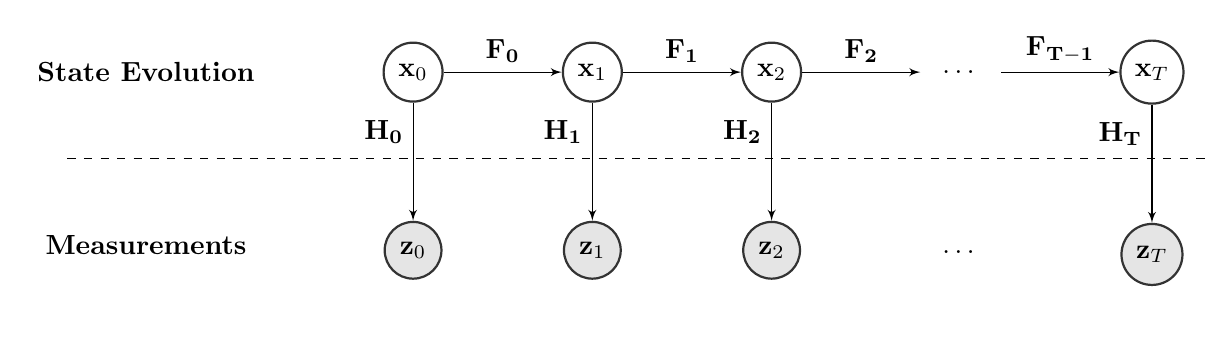
\begin{tikzpicture}[edge/.style = {->,> = latex'}]
\node[box,draw=white!100] (Latent) {\textbf{State Evolution}};
\node[main] (L1) [right=of Latent] {$\mathbf{x}_0$};
\node[main] (L2) [right=of L1] {$\mathbf{x}_1$};
\node[main] (L3) [right=of L2] {$\mathbf{x}_2$};
\node[invis] (L4) [right=of L3] {};
\node[main] (Lt) [right=of L4] {$\mathbf{x}_T$};
\node[main,fill=black!10] (O1) [below=of L1] {$\mathbf{z}_0$};
\node[main,fill=black!10] (O2) [below=of L2] {$\mathbf{z}_1$};
\node[main,fill=black!10] (O3) [below=of L3] {$\mathbf{z}_2$};
\node[invis] (04) [below=of L4] {};
\node[main,fill=black!10] (Ot) [below=of Lt] {$\mathbf{z}_T$};
\node[box,draw=white!100, below=of Latent, yshift=-7mm] (Observed) {\textbf{Measurements}};
\path (L3) to node {\dots} (Lt);
\draw[edge] (L1) to node[above] {$\mathbf{F_0}$} (L2);
\draw[edge] (L2) to node[above] {$\mathbf{F_1}$} (L3);
\draw[edge] (L3) to node[above] {$\mathbf{F_2}$} (L4);
\draw[edge] (L4) to node[above] {$\mathbf{F_{T-1}}$} (Lt);
\path (O3) to node {\dots} (Ot);
\draw[edge] (L1) to node[near start, left] {$\mathbf{H_0}$} (O1);
\draw[edge] (L2) to node[near start, left] {$\mathbf{H_1}$} (O2);
\draw[edge] (L3) to node[near start, left] {$\mathbf{H_2}$} (O3);
\draw[edge] (Lt) to node[near start, left] {$\mathbf{H_T}$} (Ot);

% draw the dashed line
\draw [dashed, shorten >=-1cm, shorten <=-1cm]
($(Latent)!0.5!(Observed)$) coordinate (a) -- ($(Lt)!(a)!(Ot)$);
\end{tikzpicture}
\caption{\textbf{The KF as a Graphical Model} - In general  $x_t \in \mathbb{R}^n$denotes the detection at time $t$, $z_t \in \mathbb{R}^m$ the measurement at $t$, $F \in \mathbb{R}^{n \times n}$ models the dynamics in the state space and $H \in \mathbb{R}^{m \times n}$ is the measurement function. The variables are assumed to be gaussian distributed with $x_{t+1} \sim \mathcal{N}(Fx_t, Q_t)$ and $z_t \sim \mathcal{N}(Hx_t, R_t)$.}
\label{graphical_model}
\end{figure}

%TODO: justify choice for quaternions

This section models the process described in section \ref{data_noise} as a Kalman Filter. The observations $\mathbf{z}_t$ are infrared detections, which are ideally four 3d points. Meaning that $\mathbf{z}_t \in \mathbb{R}^{12}$. However due to FPs and FNs this is not always the case. How these cases are handled is described in \ref{heuristics}. For now let's assume  $\mathbf{z}_t \in \mathbb{R}^{12}$. \\
The corresponding state $\mathbf{x}_t)$ holds the quantities to be estimated, which are the current position, $\mathbf{p}_t = (p_x, p_y, p_z)^T \in \mathbb{R}^4$ and orientation, $\mathbf{q}_t=(q_w, q_x, q_y, q_z)^T \in \mathbb{R}^4$ expressed as a quaternion, %TODO where to explain quaternions? 
as well as the current velocity, $\mathbf{v}_t=(v_x, v_y, v_z) \in \mathbb{R}^3$. This that this Kalman Filter assumes a constant velocity model for the position estimation and a brownian motion model for the orientation estimation. %TODO explain why I chose so, and google if there are better alternatives.

The state is $\mathbf{x}_t = (p_x, p_y, p_z, v_x, v_y, v_z, q_w, q_x, q_y, q_z)^T$.
The linear state transition function is 

$F =
\begin{pmatrix}
1 & 0 & 0 & 1 & 0 & 0 & 0 & 0 & 0 & 0 \\
0 & 1 & 0 & 0 & 1 & 0 & 0 & 0 & 0 & 0 \\
0 & 0 & 1 & 0 & 0 & 1 & 0 & 0 & 0 & 0 \\
0 & 0 & 0 & 1 & 0 & 0 & 0 & 0 & 0 & 0 \\
0 & 0 & 0 & 0 & 1 & 0 & 0 & 0 & 0 & 0 \\
0 & 0 & 0 & 0 & 0 & 1 & 0 & 0 & 0 & 0 \\
0 & 0 & 0 & 0 & 0 & 0 & 1 & 0 & 0 & 0 \\
0 & 0 & 0 & 0 & 0 & 0 & 0 & 1 & 0 & 0 \\
0 & 0 & 0 & 0 & 0 & 0 & 0 & 0 & 1 & 0 \\
0 & 0 & 0 & 0 & 0 & 0 & 0 & 0 & 0 & 1 \\
\end{pmatrix}
$
$F$ models the dynamics of a constant velocity model for the position estimation and a brownian motion model for the orientation estimation. 

The measurement function $H$ mapping from state space to measurement space is unfortunately not linear anymore. The problem is the inherent non-linearity of rotations. Whereas a fixed rotation is a linear operation, the rotation becomes non-linear when the parameters describing the rotation are seen as variables, which is exactly the case here. \\
The non-linear version of the measurement function $h: \mathbb{R}^{10} \rightarrow \mathbb{R}^{12}, (\mathbf{p}, \mathbf{v}, \mathbf{q})^T \mapsto \text{Rot}(\mathbf{q})\mathbf{p}$, where $\text{Rot}(\mathbf{q})$ denotes the rotation matrix, which describes the same rotation as the quaternion $\mathbf{q}$. See appendix \ref{quat_to_mat} for details. \\
The Extended Kalman Filter (EKF) is a simple extension of the simple KF, which can handle non-linear state-transition functions and non-linear measurement functions, by approximating them with their Jacobians. The Jacobian is locally the best linear approximation to a non-linear function. This approximation can deteriorate the performance of the EKF, when very non-linear functions are used. %TODO investigate measurement function H and state why linear approximation is OK in this case.

$Q_t$ is the covariance matrix of the process noise and $R_t$ is the covariance matrix for the measurement noise.

In total this amounts to the following equations describing the system:

$\mathbf{x}_{t+1} = F\mathbf{x}_t + \mathbf{w}_t$, where $\mathbf{w}_t \sim \mathcal{N}(0, Q_t)$.

$\mathbf{z}_{t} = H\mathbf{x}_t + \mathbf{v}_t$, where $\mathbf{v}_t \sim \mathcal{N}(0, R_t)$.


\subsubsection{Data Association}
\label{heuristics}
% I applied a set of heuristics in order to tackle the data specific difficulties. as described in ref sec 2.2
As explained in \ref{kalman_filter_approach}, this is the key tasks to be performed in MOT. This component enables MOT by stringing together all the independent EKFs. The method described in the following relies heavily on heuristics and hyper-parameters. The choices made were not extensively tested. In the future this task could be done with a neural network, which works better on a large variety of possible scenarios than these handcrafted rules.

\paragraph{Detection to Track Assignment} 
The first step is to do the detection to \emph{track} assignment. This is just a small preprocessing step to make the \emph{detetion to marker assignment} easier. The optimal assignment is calculated with a version of the Hungarian Algorithm, which additionally allows unassigned tracks and unassigned detections. The assignment costs are based on the distances of the predicted marker locations to the detections. The cost of not assigning a detection to any track and not assigning any detection to a track is set to 50. As the pairwise distances of the points in a pattern are roughly ranging between 15 and 50, this is a bit generous and will tend to sometimes assign FPs to a track if there are some FNs. Experiments showed that setting a lower value, will lead the system to lose tracks, when the constant velocity model of the Kalman Filter fails to predict a precise position for the next frame. Setting the cost for non-assignments too high will sometimes cause multiple FPs assigned to a track. This renders the algorithm explained in the next paragraph inefficient, since it considers all permutations of the detections assigned to a single track.

\paragraph{Filtering false positives} %TODO

\paragraph{Detection to Marker Assignment}
\label{dtma}
When there are 2 or less detections assigned to a track, there is not enough information to reason about the orientation of the pattern. Then the assignment to markers is solely based on the predicted marker locations, exactly as in the \emph{detection to track assignment}.\\
If there are 3 or more detections assigned to a track, the structure of these three detections can give clues about the orientation of the pattern. This case is handled with a simple brute-force method, which calculates costs for every possible detection to marker assignment. The costs are composed of 4 parts:
\begin{equation}
\begin{split}
 \text{cost(pattern, det)} \quad = \quad  ~ \text{MSE}\left(\texttt{pdist}(\text{pattern}) - \texttt{pdist}(\text{det}) \right)  \qquad \qquad \qquad \qquad \qquad \quad \\
  +\quad \lambda \cdot \text{MSE}\left( \texttt{pangles}(\text{pattern}) - \texttt{pangles}(\text{det}) \right) \qquad \qquad \qquad ~~ \\
  +\quad \text{MSE}\left(\texttt{rot}(\text{pattern},\hat{q}_t) - det\right) \quad \qquad \qquad \qquad \qquad \qquad \quad ~\\
  +\quad \texttt{costOfNonAssignment} \cdot \#(\text{non-assignments}) \quad \qquad \qquad \quad
\end{split}
\end{equation}

, where \emph{pattern} are the 4 markers ordered by one of the permutations, \emph{det} are the detections, \texttt{pdist} and \texttt{pangles} are functions calculating the all pairwise distances and angles respectively,  \texttt{rot} rotates pattern as described by $\hat{q}_t$, and $\#(\text{non-assignments})$ are the number of detections which were not assigned to a marker. The permutations are calculated such that it is possible to not assign all but 3 markers. $\lambda$ and \texttt{costOfNonAssignment} are two more hyperparameters to balance the influences of the parts.

\paragraph{Adapting the noise} %TODO

\subsubsection{Track Management Unit}
This part of the system reasons about the death and birth of tracks. %TODO new paragraph for death as well?
The death of tracks is governed by one rule  only. This rule removes track which were not assigned any detections for more than \texttt{invisibleForTooLong=20} many frames.

\paragraph{Creating New Tracks}  %TODO: before using umeyama, you need to determine assignment as before!
Since ID-switches are to be avoided, new tracks are only created if there are 4 detections that match a pattern of an untracked bird close to exact. The unassigned detections are clustered based on distances. The matching of such a cluster detections with a pattern is done with the method developed in \cite{umeyama}. This method finds the optimal (with respect to least square error) rotation, translation and scaling transformations to transform one set of m-dimensional points to match another set. As there can be many such clusters and untracked bird, the Hungarian Algorithm is applied once more. For each pair of cluster and pattern, the cost is calculated as the mean squared error output by the Umeyama matching. There is another handcrafted cost of non assigned, which is set very low in order to only create new tracks, when the detections match a pattern very close. The translation vector is used as initial position of the track and the rotation matrix is converted to a quaternion and used as initial orientation.




\subsection{Deep Learning Approach}
\label{dl_approach}

\paragraph{Potential benefits}
I believe that the main benefits of a Deep Learning approach  compareed to tha Kalman Filter approach are the following: 
\begin{enumerate}
	\item It is possible to build a more complex motion model, which can make accurate position predictions multiple steps into the future. Due to the simplicity of the motion model used in the KF, position predictions become very inaccurate very quickly. Good long-term trajectory predictions can potentially reduce the number of lost tracks in periods, when detections are missing for multiple frames. The non-determinism of bird behaviour however complicates predicting future positions. In order to tackle this problem, commonly multi-model position predictions are used. Combining multi-modal predictions and long-term predictions is complicated. One solution is presented in %TODO cite dbscan traj. orediction paper
	.
	\item There is no need for an explicit \emph{detection-to-marker-assignment} in order to predict the orientation. The neural network can directly predict the position and orientation. My experiements showed that while the neural network was able to accurately predict position and orientation, it was not able to reliably assign the detections to the markers, as presented in section \ref{results_dl}. 
\end{enumerate} 

% TODO Differences to common models here or in section 2????
\subsubsection{Generating Training Data}
\label{training_data}
%TODO write somewhere in the beginningLack of Training Data
There are no labeled bird trajectories available and labelling the data manually is so time-consuming that is infeasible to label a sufficient about for proper training. The abscence of input-to-ground-truth-pairs means, that the neural network cannot be trained on the real data and therefore will not be able to learn the intricacies of the task at hand. \\
One way of obtaining training data, is to generate sequences of 3d positions and orientations and then to simulate birds flying alon the generate positions. As it is hard to generate trajectories which mimic the bird behaviour, I resorted to a different approach. Instead of generating the 3d trajectories I use the position estimations from the kalman filter. A qualitative, visual analysis of these position predictions confirmed them to be very accurate with occasional small jumps, which I erased with a moving median filter. The orientation predictions are to noisy to be directly used for the training data. %TODO think about quat generation and write down
The critical part however is mimicing the noise present in the data, as false positives and false negatives are the main difficulty. Observing the false negatives and positives reveal some patterns which I tried to represent with two noise models, in order to stay as close to the real data as possible.
%TODO: explain analysis of FN noise behvaiour and FP noise behaviour
%TODO: describe noise generation methods

This approach seemed to be the best compromise to stay as close to the real data as possible, while being able to obtain enough training data to effectively train the network.

%TODO: random 3d trajectories to verify appraoch??

%TODO: maybe dilemma, KF very good-> good training data but no need for NN. KF bad, no training data but need for NN


\subsubsection{Own Model Architecture}

\subsubsection{Training Details}
%TODO: mention google colab


\subsubsection{How to Improve the Model}

\section{Results}
\label{results}

In order to evaluate the effectiveness of the models, I used the method described in \ref{training_data} to generate data with known ground truth. Doing so allows to specifiy the level of noise present in the data, which enables a to analyize the noise robustness of the different methods and evaluate the design decision in a more detailed way. Additionally I did a qualitative comparison between our models and the VICON TRACKER3 results in section \ref{comparison_vicon}, since a quantitative analysis is impossible for the lack of ground truth.

\subsection{Kalman Filter}
\label{results_kalman_filter}

\subsection{Deep Learning Approach}
\label{results_dl}

%TODO: intersting observation: estimation quality gets worse when moving away from the origin, reason? A) not enough training data for such situations, B) numbers get too large for NN?



\subsection{Qualitative Comparison to VICON}
\label{comparison_vicon}

\section{Future Work}
%TODO explain detection to track assignemnt in related work
% TODO explain detecton to marker assignemnt later on!
%TODO nochmal proof readen, shr sloppy geschrieben
The solid performance of the Kalman Filter approach shows that a simple position prediction method, like a constant velocity model, is enough in most cases to maintain the tracks over time and inhibit ID-switches. Since the position of birds does not change drastically within a single time step, the detection to track assignment, which is the most critical step in MOT, is relatively easy. However the exact detection to marker assignment is harder already. However an exact detection to marker assignment is not strictly necessary, since error introduced by such are quite small. \\
There are however two major difficulties that remain:
First, orientation estimation is especially challenging because small mistakes in the detection to marker assignment or an undetected FP can completely disrupt the estimation. This problem could be tackled with better heuristics Since coming up with viable heuristics can be very tedious, a Neural Network could be trained to handle the detection to marker assignment. Such an approach will be subject of future research.\\
Secondly long term predictions are are required to fill gaps in cases with no or very few detections for multiple consecutive frames. As \cite{tracking_the_trackers} found, most MOT algorithms increase the FN rate, instead of decreasing it by filling in gaps. This leads to the conclusion that \emph{trajectory prediction literature} seems more promising than \emph{MOT literature} to tackle the problem at hand. Since even the simple constant velocity motion model of the EKF was sufficient to produce good position estimation and inhibit any ID-switches, it seems reasonable to disregard the tracking of multiple objects, focus on good trajectory prediction and obtain MOT by the Hungarian Algorithm and simple heuristics to manage the birth and death of tracks.

\section{Summary}

\begin{figure}[ht]
	\centering
	\begin{minipage}{.7\linewidth}
		%TODO new names nlset{}
		
		\begin{algorithm}[H]
			\DontPrintSemicolon
			\KwData{$G=(X,U)$ such that $G^{tc}$ is an order.} %TODO
			\KwResult{$G’=(X,V)$ with $V\subseteq U$ such that $G’^{tc}$ is an %TODO
				interval order.}
			\Begin{
				\nl Initialize tracks \;
				\For{$d\in D$}{
					\nlset{predict()} KF predict step \; %TODO for eacvh active track do predict
					\nlset{detectionToMarkerAssignment()} Assign detections to markers\; \label{detection_to_marker_assignment} %TODO details later
					\nlset{correct()} KF correct step \; % TODO fora each actove track correct()
					\nlset{deleteTracks()} Decide if tracks were lost \; %TODO give details here
					\nlset{createTrcks()} Create new tracks if pattern could be found in unassigned detections \; %TODO details later
				}
			}
			\caption{MOT with multiple KFs} %TODO
			
		\end{algorithm}
		
	\end{minipage}
\end{figure}

\bibliographystyle{apalike}  
\bibliography{references}

\begin{appendices}

\section{Quaternions}
\subsection{From Quaternions to Rotation Matrices}
\label{quat_to_mat}
% TODO


\end{appendices}


\end{document}
